

\section{Master-Worker Algorithm for two processes}

\begin{figure}[ht]
  \centering{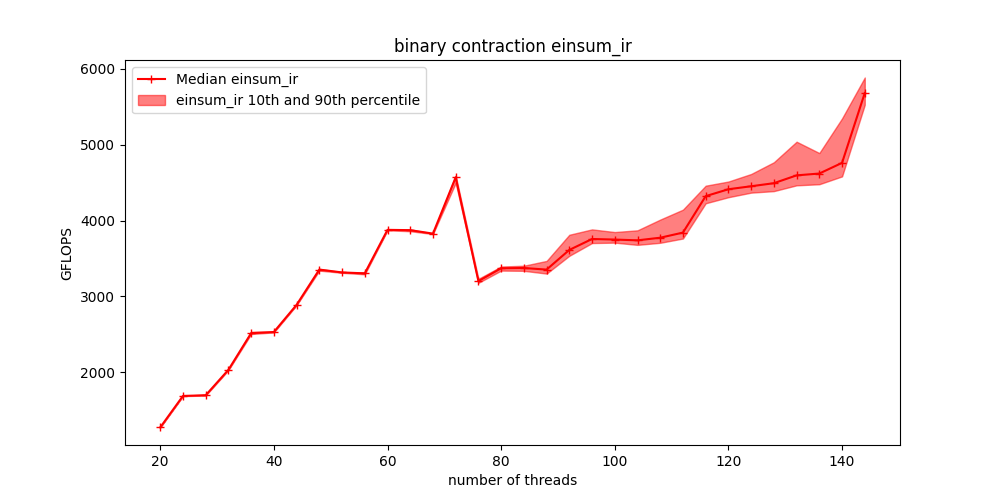
\includegraphics[width=0.95\textwidth]{gflops_threads.png}}
  \caption{
    Performance of einsum\_ir on an Nvidia Grace CPU Superchip.
    Grace consists of two 72-core CPUs connected via NVLink.
    The contraction used is $m_0c_0k_0k_1m_1, n_0c_0k_0n_0n_1 \rightarrow m_0n_0c_0n_1m_1$ with $|c_0|=2$, $|m_0|=|n_0|=|k_0|$ and $|m_1|=|n_1|=|k_1|=70$.
  }
  \label{fig:perf_threads}
\end{figure}

\texttt{einsum\_ir} is scaling well across a single NUMA domain as seen in Figure \ref{fig:perf_threads} before 72 threads.
As soon as a second NUMA domain gets included, in the Figure \ref{fig:perf_threads} after 72 threads, the performance drops significantly.
Even at 144 threads the performance is only improved by 24\%.

As a first algorithm we will think of a master worker architecture to improve performance across NUMA domains.
Since the main hardware target were dual socket servers, like the Nvidia Grace CPU Superchip, we will restrict our algorithm to two processes.
The basic premise of this algorithm is treating the worker as a matrix accelerator where you send parts of the input matrix too and receive the corresponding parts of the output matrix back.
Since both NUMA domains should ideally be equally fast we will cut all tensor across one dimension c dimension $c_0$ into $|c_0|$ chunks with the master working on the first $\frac{|c_0|}{2}$ as one big contraction and will send the worker thread $|c_0|-\frac{|c_0|}{2}$ single chunks to process.
To enable the overlap of communication with the other process and contracting the chunks each process uses one of its thread exclusively as communication thread.
This thread will be solely responsible for communicating the array chunks to each other.

From the perspective of the master thread no synchronization between computation and communication threads has to occur.
The worker threads compute threads however have to wait until their input data is fully assembled before they can start working.
To minimize the waiting times the computation and communication will go as follows, $A_i$, $B_i$ and $C_i$ will each be the $i$-th chunk contracted on the worker:

\begin{center}
  \begin{tabular}{ |c|c| } 
  \hline
  compute threads & communication thread\\
  \hline
   & \texttt{receive} $A_1$ and $B_1$\\
  \hline
  $A_1,B_1 \rightarrow C_1$ & \texttt{receive} $A_2$ and $B_2$\\
  \hline
  $A_2,B_2 \rightarrow C_2$ & \texttt{receive} $A_3$ and $B_3$\\
  & \texttt{send} $C_1$\\
  \hline
  \multicolumn{2}{|c|}{\dots}\\
  \hline
  $A_k,B_k \rightarrow C_k$ & \texttt{receive} $A_{k+1}$ and $B_{k+1}$\\
  & \texttt{send} $C_{k-1}$\\
  \hline
  \multicolumn{2}{|c|}{\dots}\\
  \hline
  $A_n,B_n \rightarrow C_n$ & \texttt{send} $C_{n-1}$\\
  \hline
  & \texttt{send} $C_n$\\
  \hline
\end{tabular}
\end{center}

The communication thread of the master matches each \texttt{receive} of the worker with a \texttt{send} and each \texttt{send} of the worker with a \texttt{receive}.
The workers compute threads have to synchronize with its communication thread after each row.
To minimize the initial memory allocation on the worker it will only have 2 buffers for each $A$, $B$ and $C$ chunks.
This is possible since all $A$ and $B$ chunks are only used in the next step after they are received and all $C$ chunks are sent in the next chunk after they are contracted.
The time in the contraction where the worker does not use its compute threads takes only as long as the time to communicate a chunk of each $A$, $B$ and $C$ (the first and last row in the table), so this time gets reduced the larger $|c_0|$ is.
It should be noted that the $|c_0|$ dimension has to be the outermost dimension of $A$, $B$ and $C$ in the implementation I developed.
This is caused by the restriction in the binary contraction interface to only work on contiguous memory as noted in \ref{sec:einsum_ir}.
To fix this limitation the contraction interface would need to support strided arrays, for example by supplying a pointer and the starts and offsets for each dimension.
The MPI calls would also need to be adjusted to a custom datatype instead of sending contiguous chunks.
